\section{About the process }

August - December 2020, the first semester on the master degree was spent finding a supervisor and deciding/ orienting on what I wanted to write about. The second semester was for the most part theoretical, getting to know the museum domain and working on the research question and angle for the thesis. Started 

\begin{figure}[h]
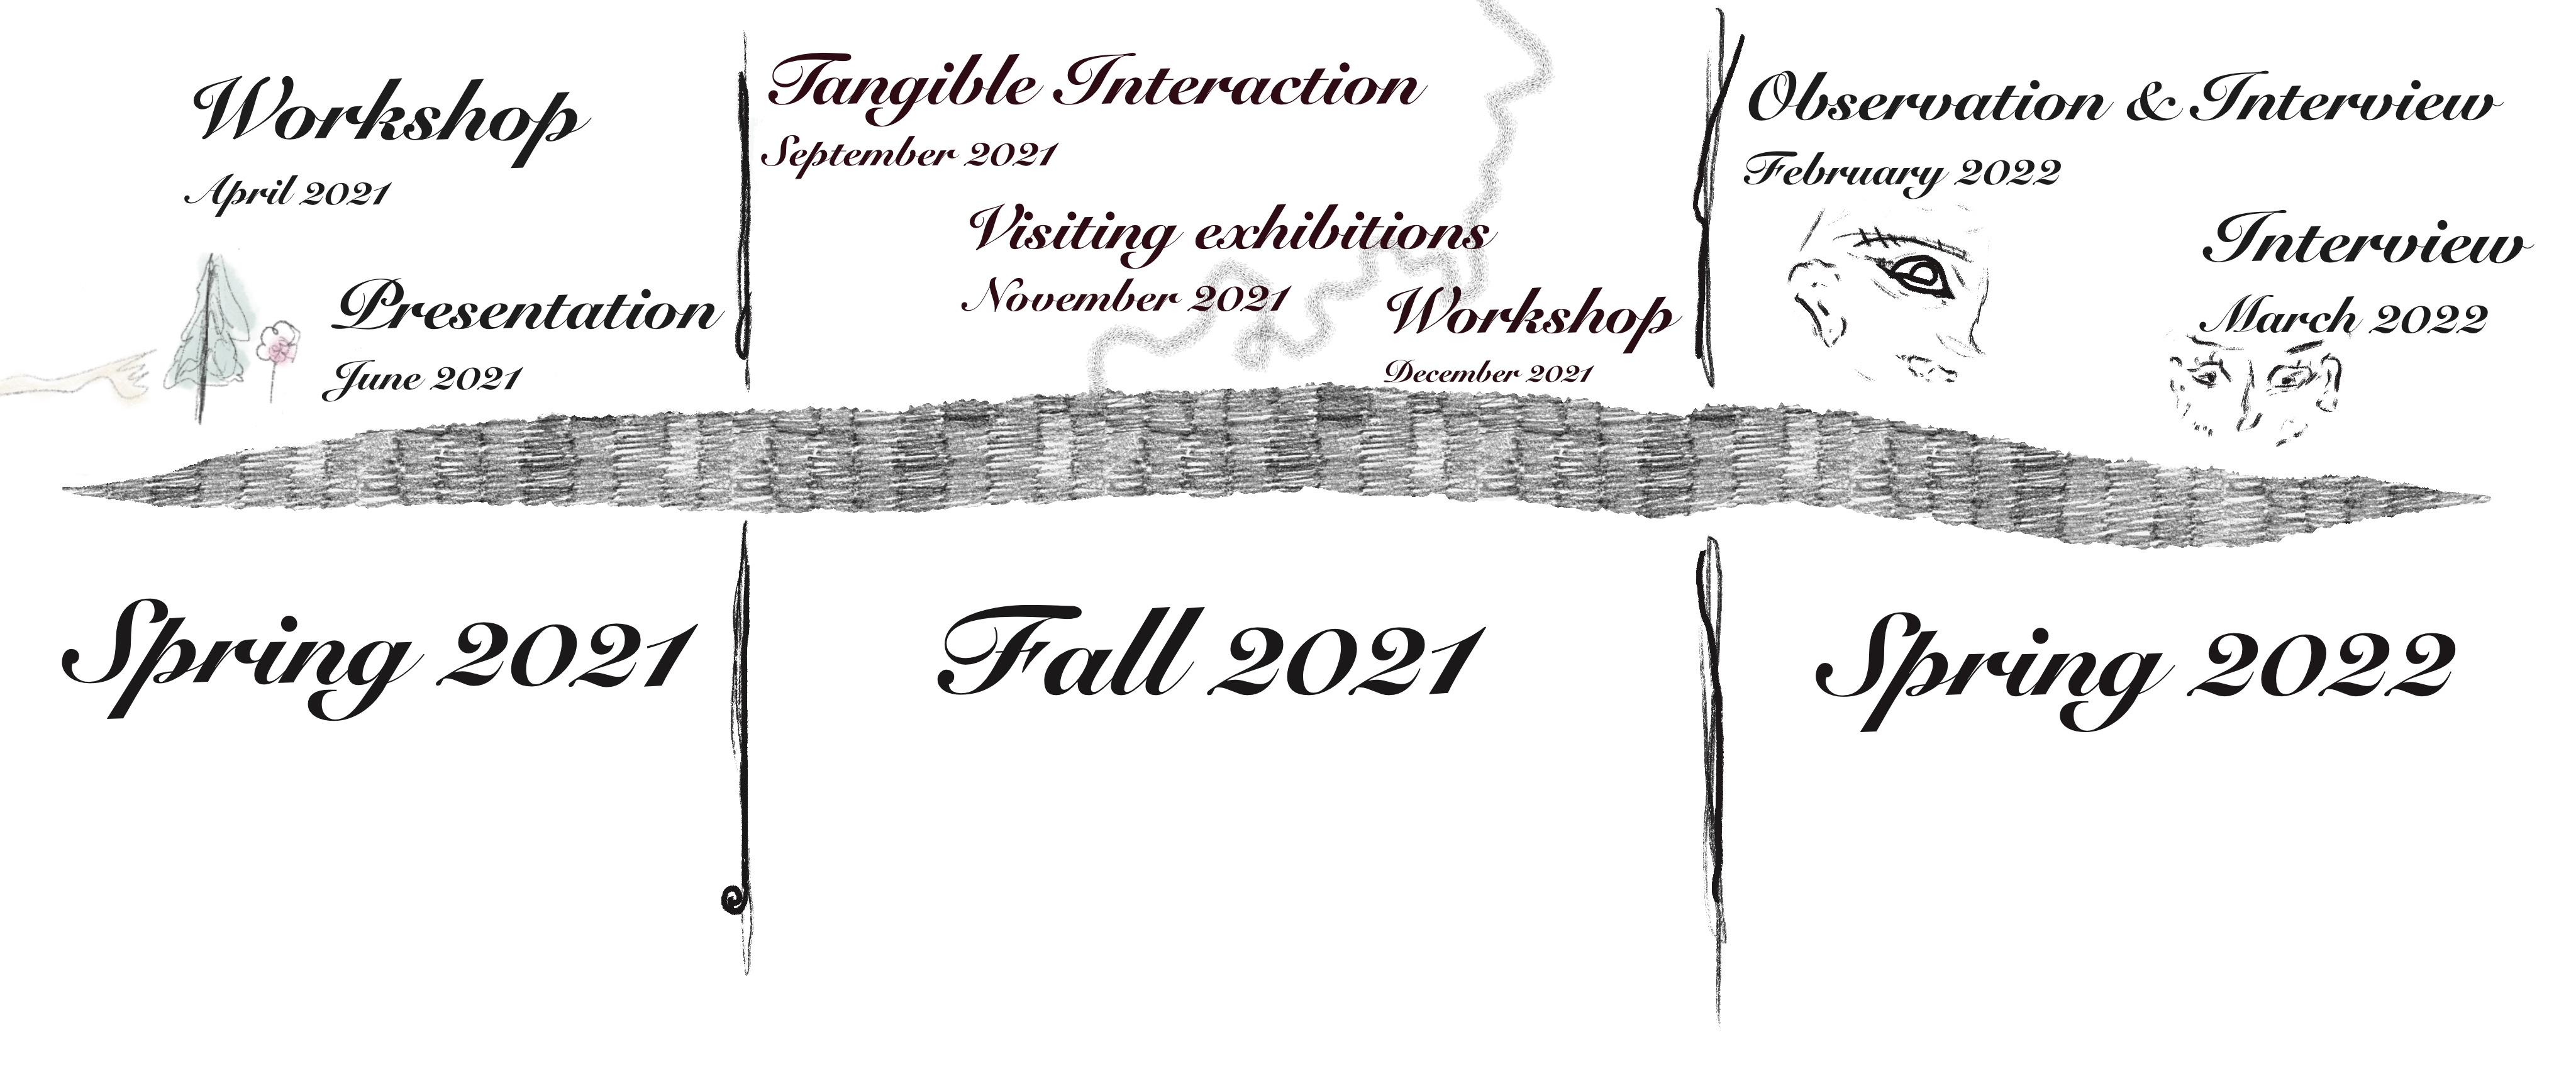
\includegraphics[width=13cm]{pictures/timeline.jpg}
\centering 
\end{figure}


The dataset that I/we have done for this thesis is as following:
\begin{itemize}
    \item Workshop with stakeholders from Klimahuset, april 21
    \item Presentation w/ prototypes at Klimahuset, june 21
    \item Visited 5 different interactive exhibitions, fall 21
    \item Energy visualisation workshop with Qi-installation
    \item Observation of 2 school children classes in Klimahuset, february 22
    \item Interview with two of Klimahuset Docents, february 22
    \item Interview and observation w/ concept developer at Munch, march 22
    \item Analysis/ theorethical framework workshop sessions
\end{itemize}

\section{The dataset}
Over the course of this thesis, my research buddies and I have visited in total 10 exhibitions from 7 different museums in Oslo. From these museum visits, we have documented 22 interactive installations that forms the dataset used for analysis and similar investigations in our respective thesis's. 

\begin{figure}[H]
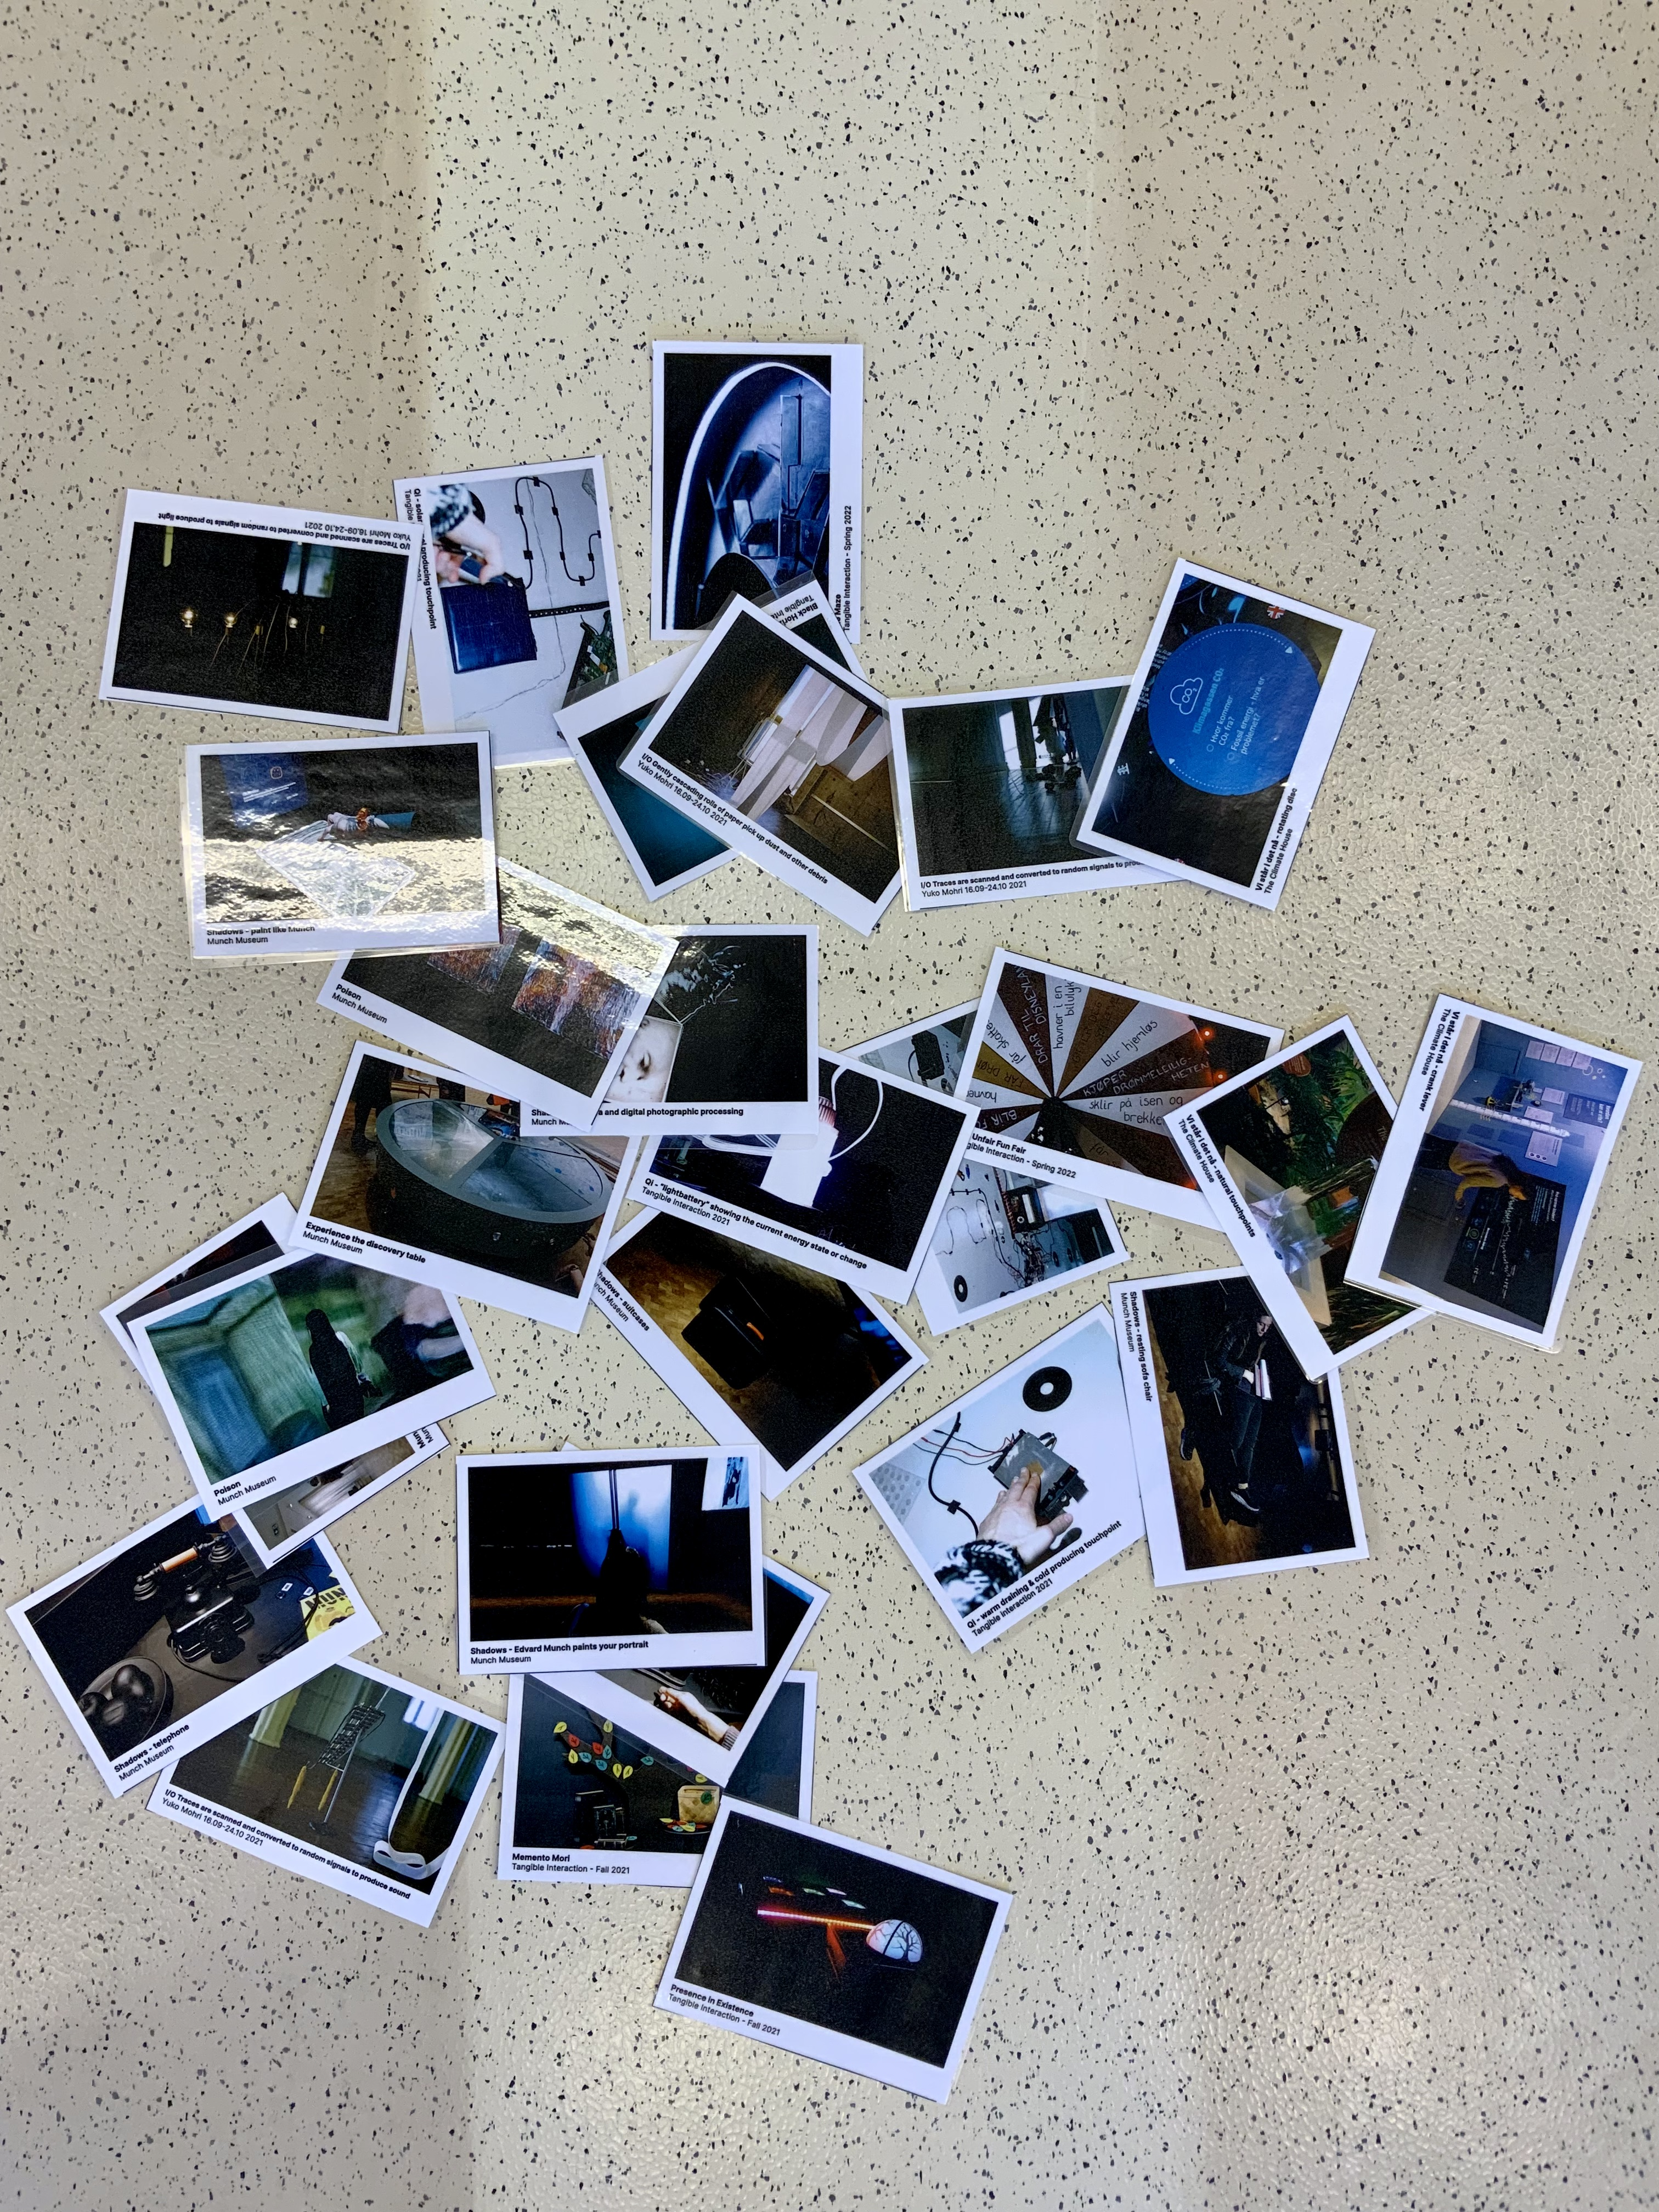
\includegraphics[width=12cm]{pictures/dataset/datasett_oversikt.jpeg}
\centering 
\end{figure}

I think this is basic qualitative analysis?

Måten jeg har gått frem på ved bruk av dette datasettet, sett opp mot mine utvalgte teorier, har vært en form for deduktiv systematisk prosess. Det vil si at jeg til å begynne med har systematisert og kategorisert installasjonene opp mot hver teori; feks som jeg har gjort her fra en av de interaktive installasjonene på klimahuset haar jeg

\subsection{"data laundering"}
Write out:
\begin{itemize}
    \item explain why munch shadows is analysed as one. and only weighted as one. and how that affects the dataset.
    \item discuss how the amount of tangible installations affect the dataset
    \item discuss the analog-tangible vs interactive-tangible installations (ice cube, munch peepholes and discovery table)
\end{itemize}

\begin{figure}[H]
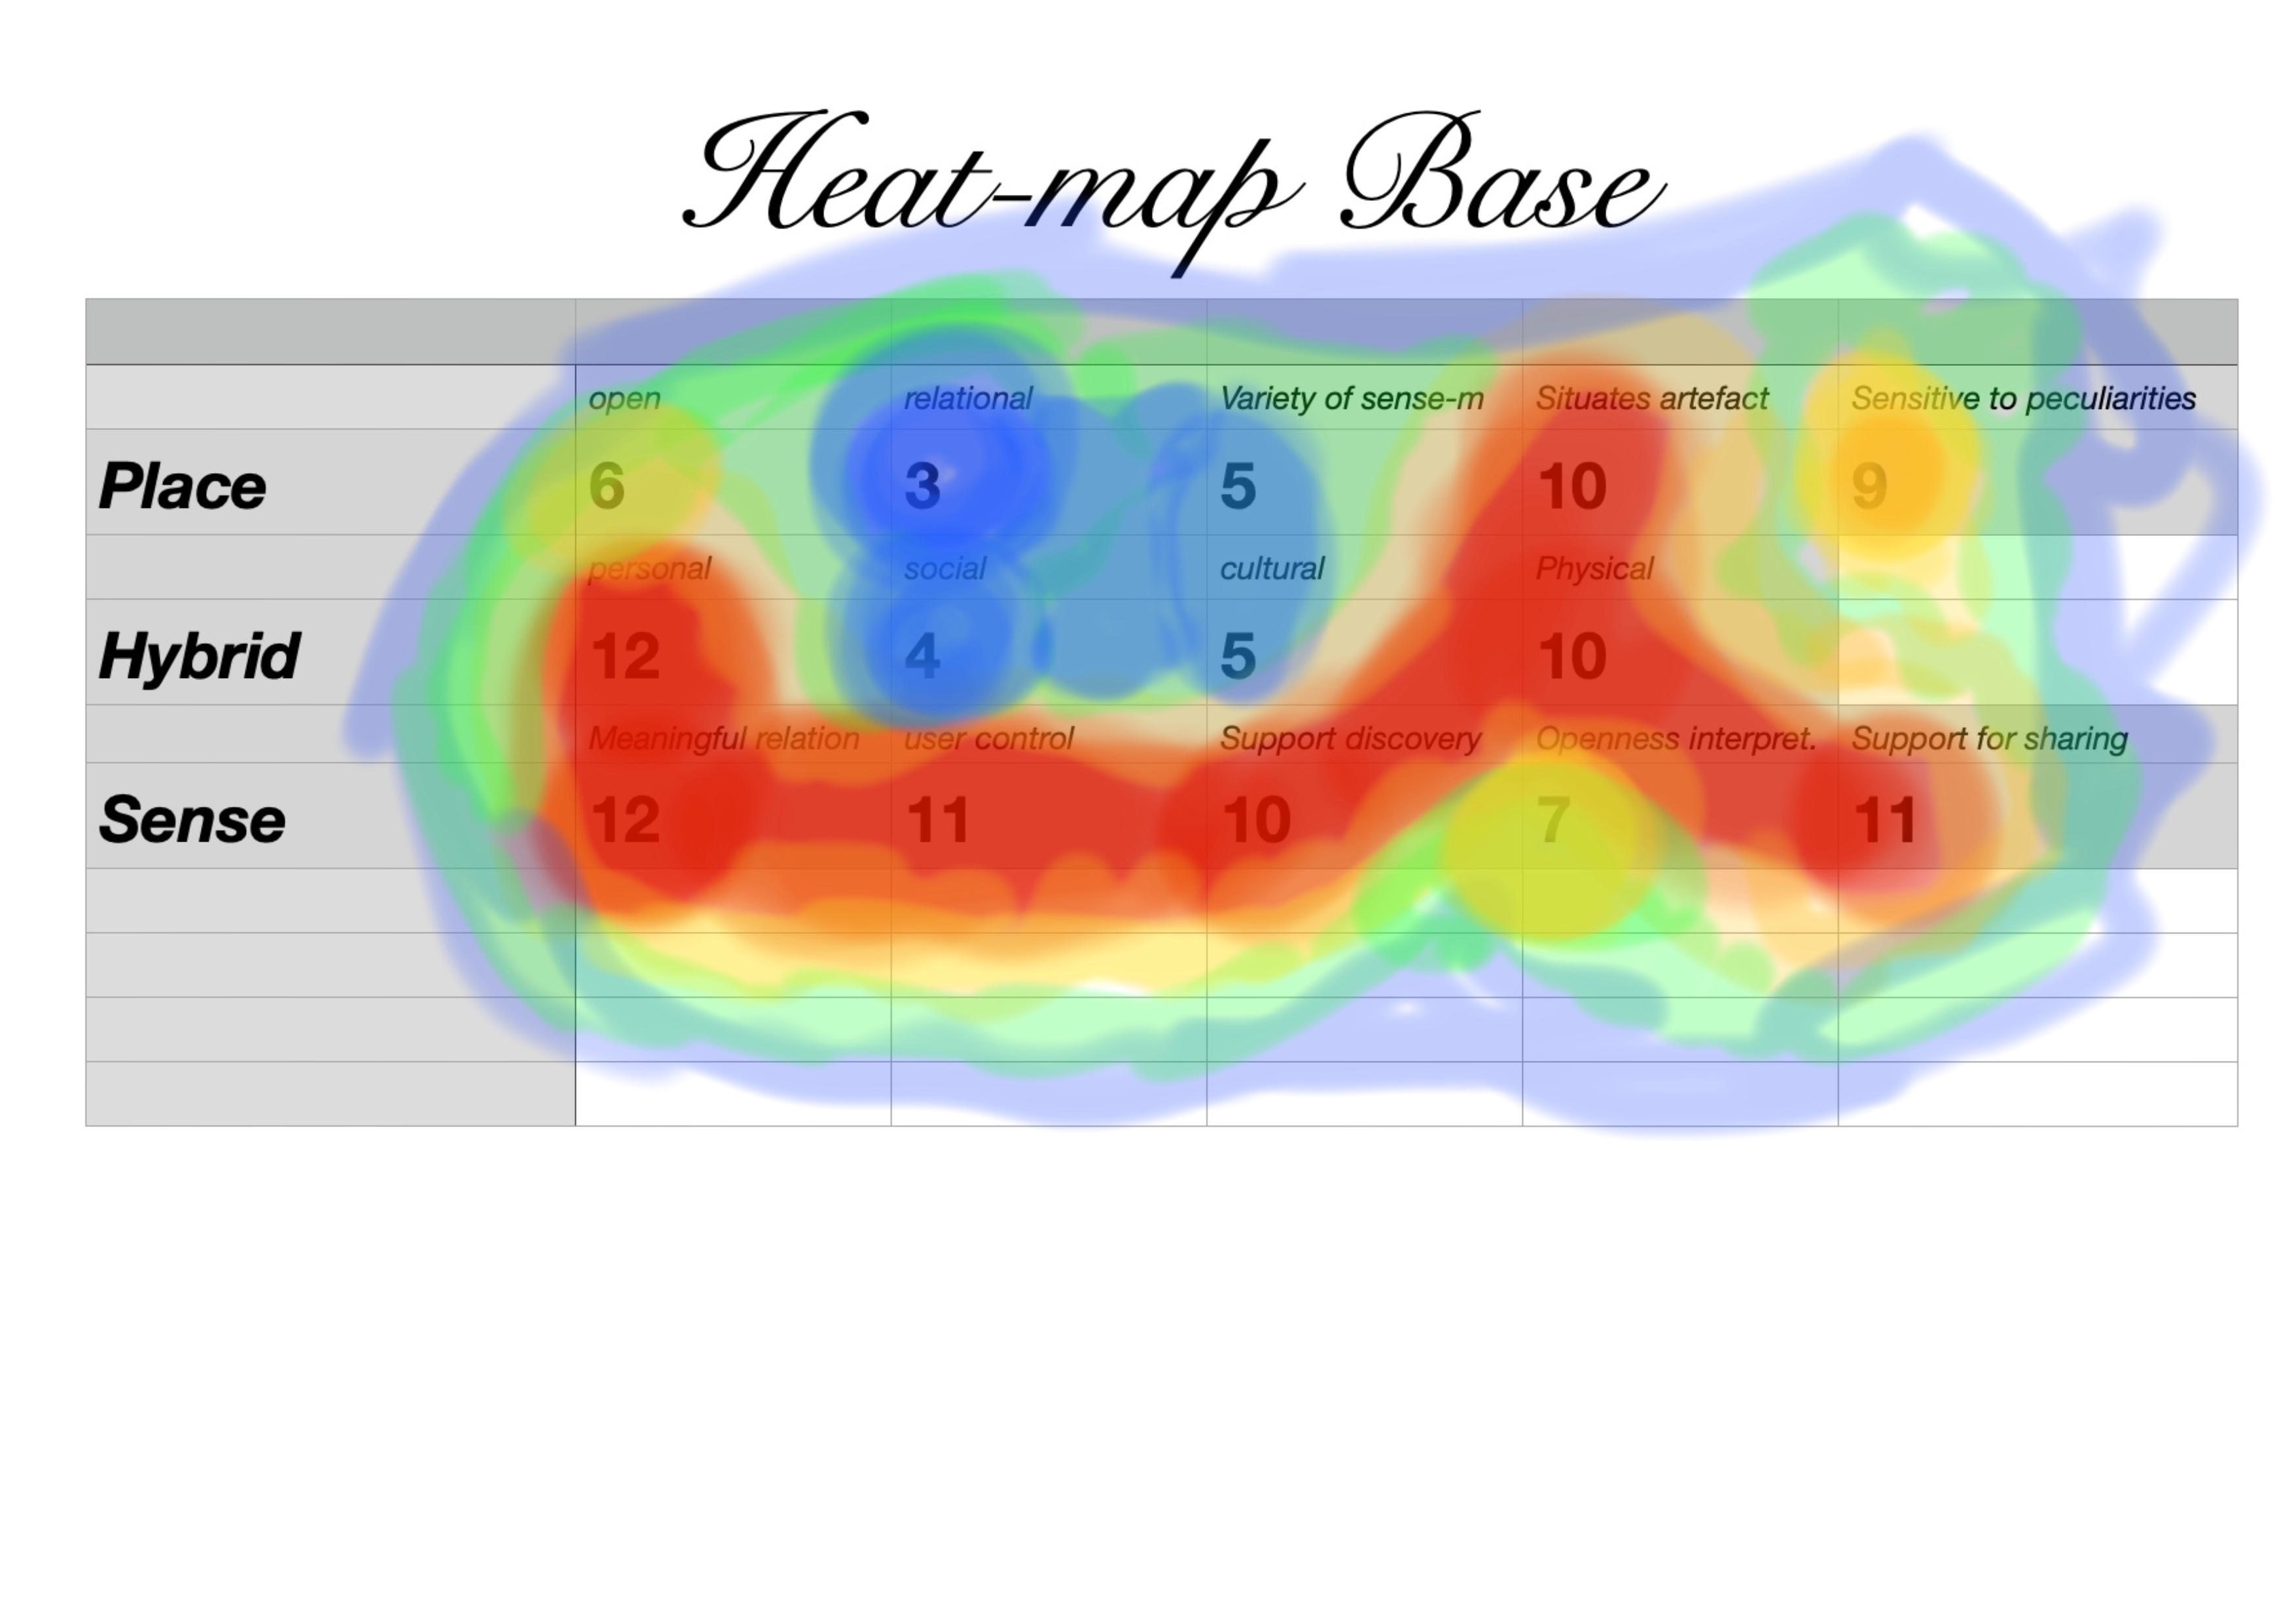
\includegraphics[width=11cm]{pictures/dataset/heatmap.jpg}
\centering 
\end{figure}


\section{First iteration: getting to know the bigger picture}

I started the first analytical iteration by sorting the dataset into the three theories I base my understanding of meaningfulness on; \emph{Hybrid place, place as a dialogue} and \emph{Sense-making strategies}. I made one table for each theory, where the frameworks's principles/ and dimensions formed the columns and the 22 different installations the rows. I then went through each installation and plotted in whether or not the installation fulfilled the principle/ dimension. Categorising it this way opened up for looking at the dataset in correlation with each theory separately, making it possible to see overall trends in the dataset according to the theories. Another


respective theory from a birds-eye, holistic, perspective, but it will also work as a quick-reference guide for the second analysis iteration when I'm trying to merge the three theories and/ or finding new relationships between the data across the theories.

The categorisation of the data is highly subjective, but theoretically grounded, based on my personal experience with- and interpretation of the installations and knowledge of the museum institution the installation was part of. I have also chosen to merge all the Munch - \emph{Shadows} installations as one, because they are a part of the same exhibition and do not differ in their interactive qualities. Because of this, the dataset used for this analysis shrinked from 22 to 16. This choice of merging the \emph{Shadows} installations was made in the process of fitting the installations into the theory's principles/ dimensions, when I saw that they all checked the same boxes. 


\begin{figure}[H]
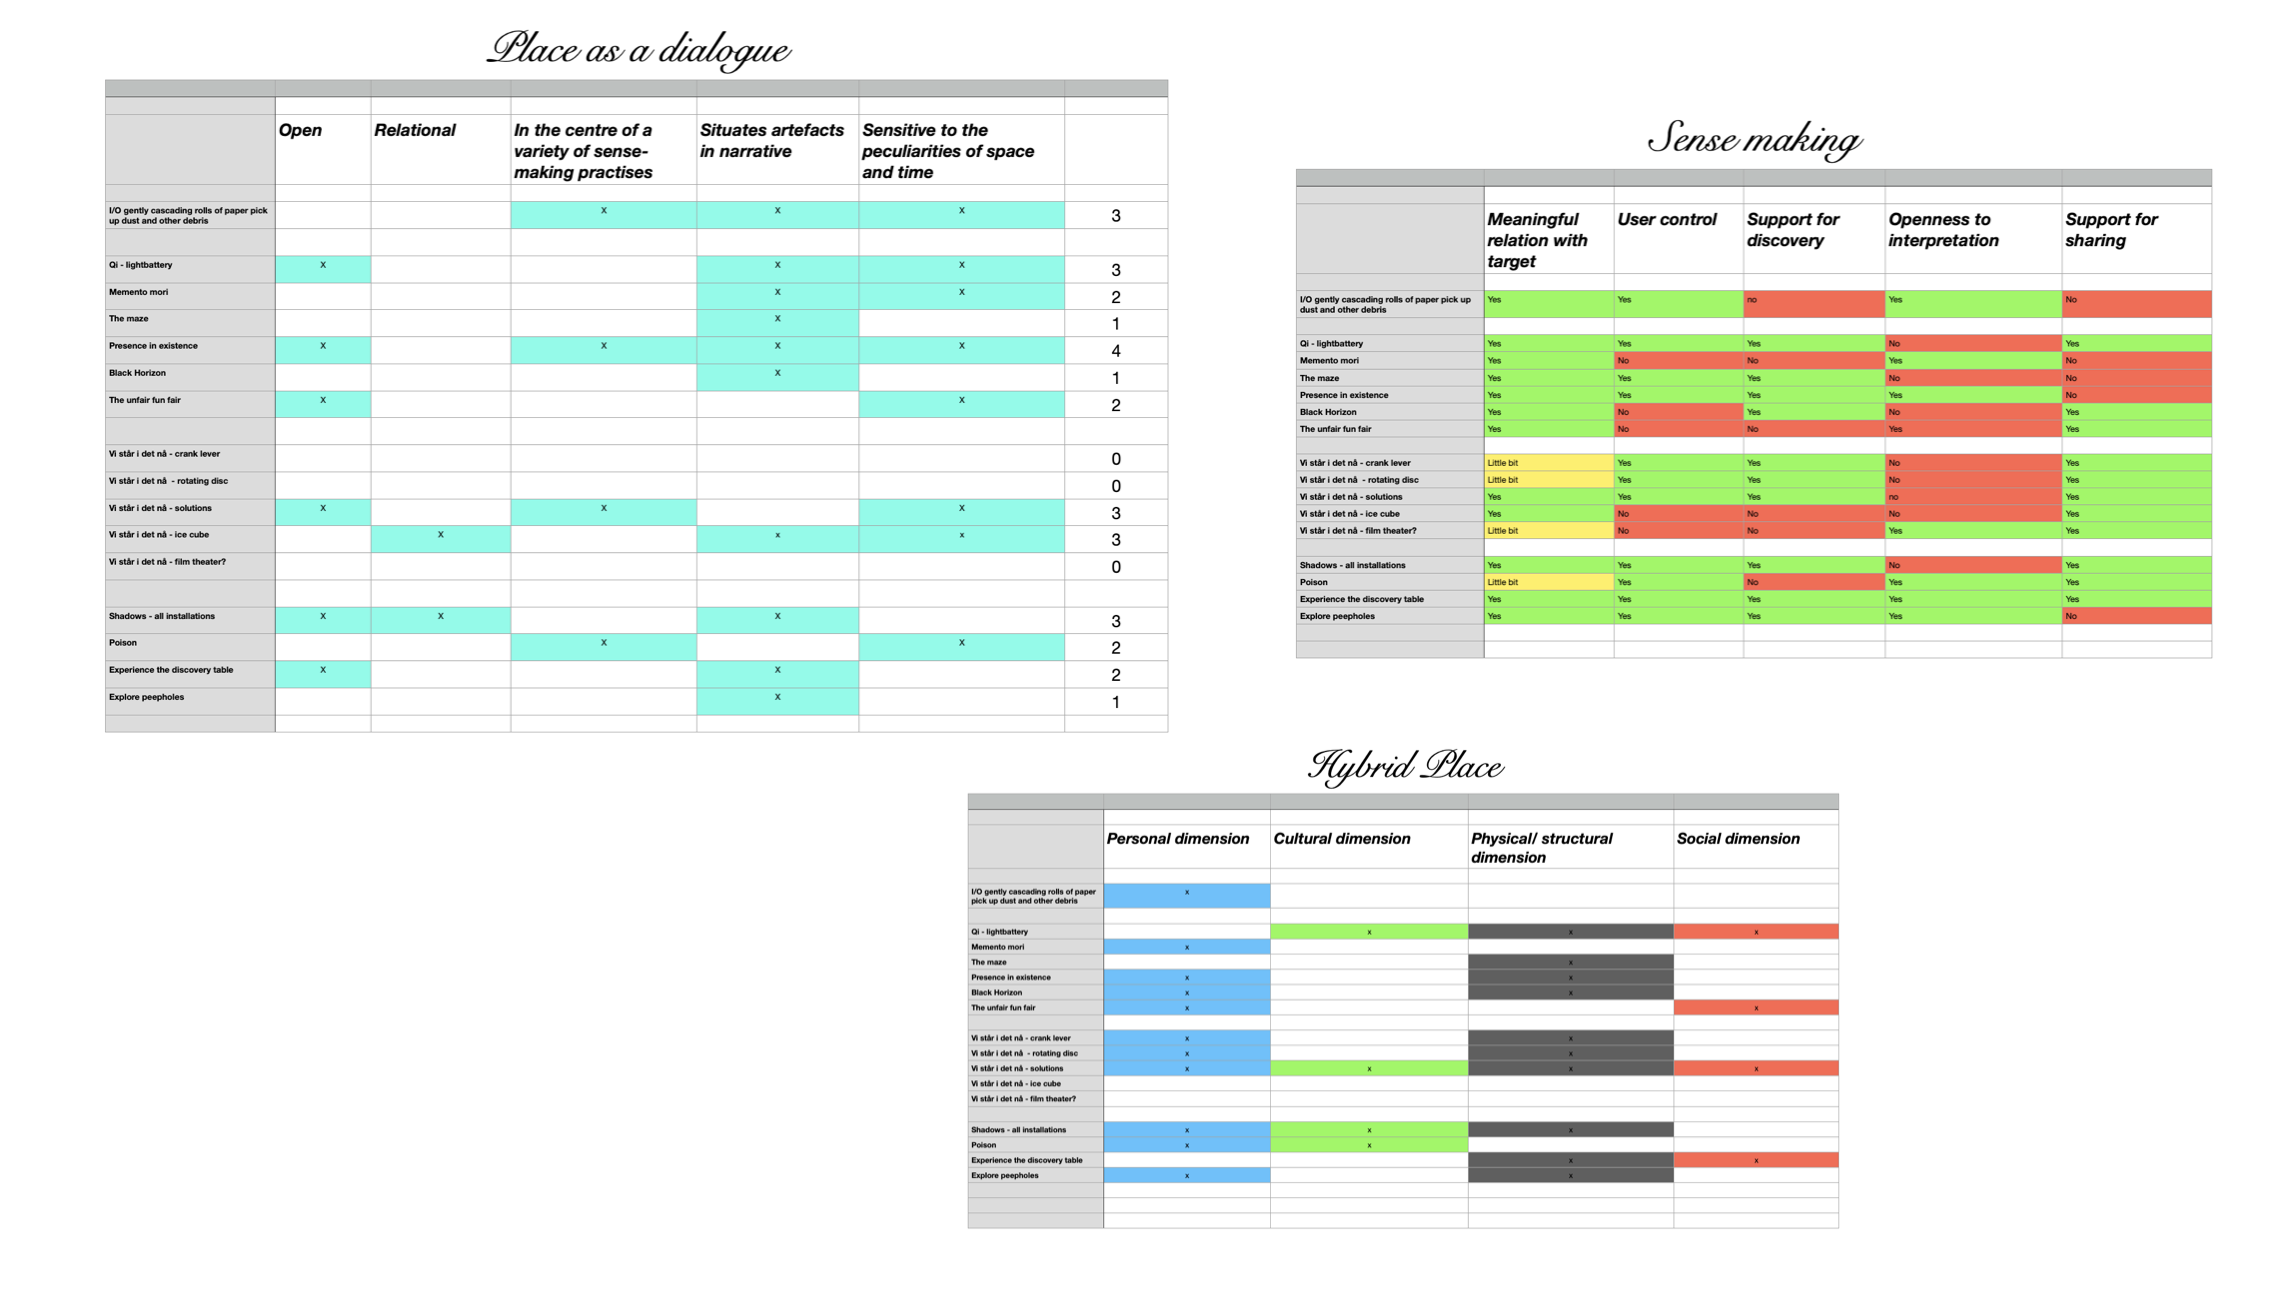
\includegraphics[width=13cm]{pictures/dataset/analysis_tables.png}
\centering 
\end{figure}

After mapping the installations in the tables, it opened up for crunching the first numbers. In this iteration I want to see the dataset from a holistic view. Abstracting from the details and seeing how the installations map up in the bigger picture. To do this I needed a diagram that could compare the different principles up against eachother. I chose to create radar charts to do this, and made a radar chart for each theory. 

\begin{figure}[H]
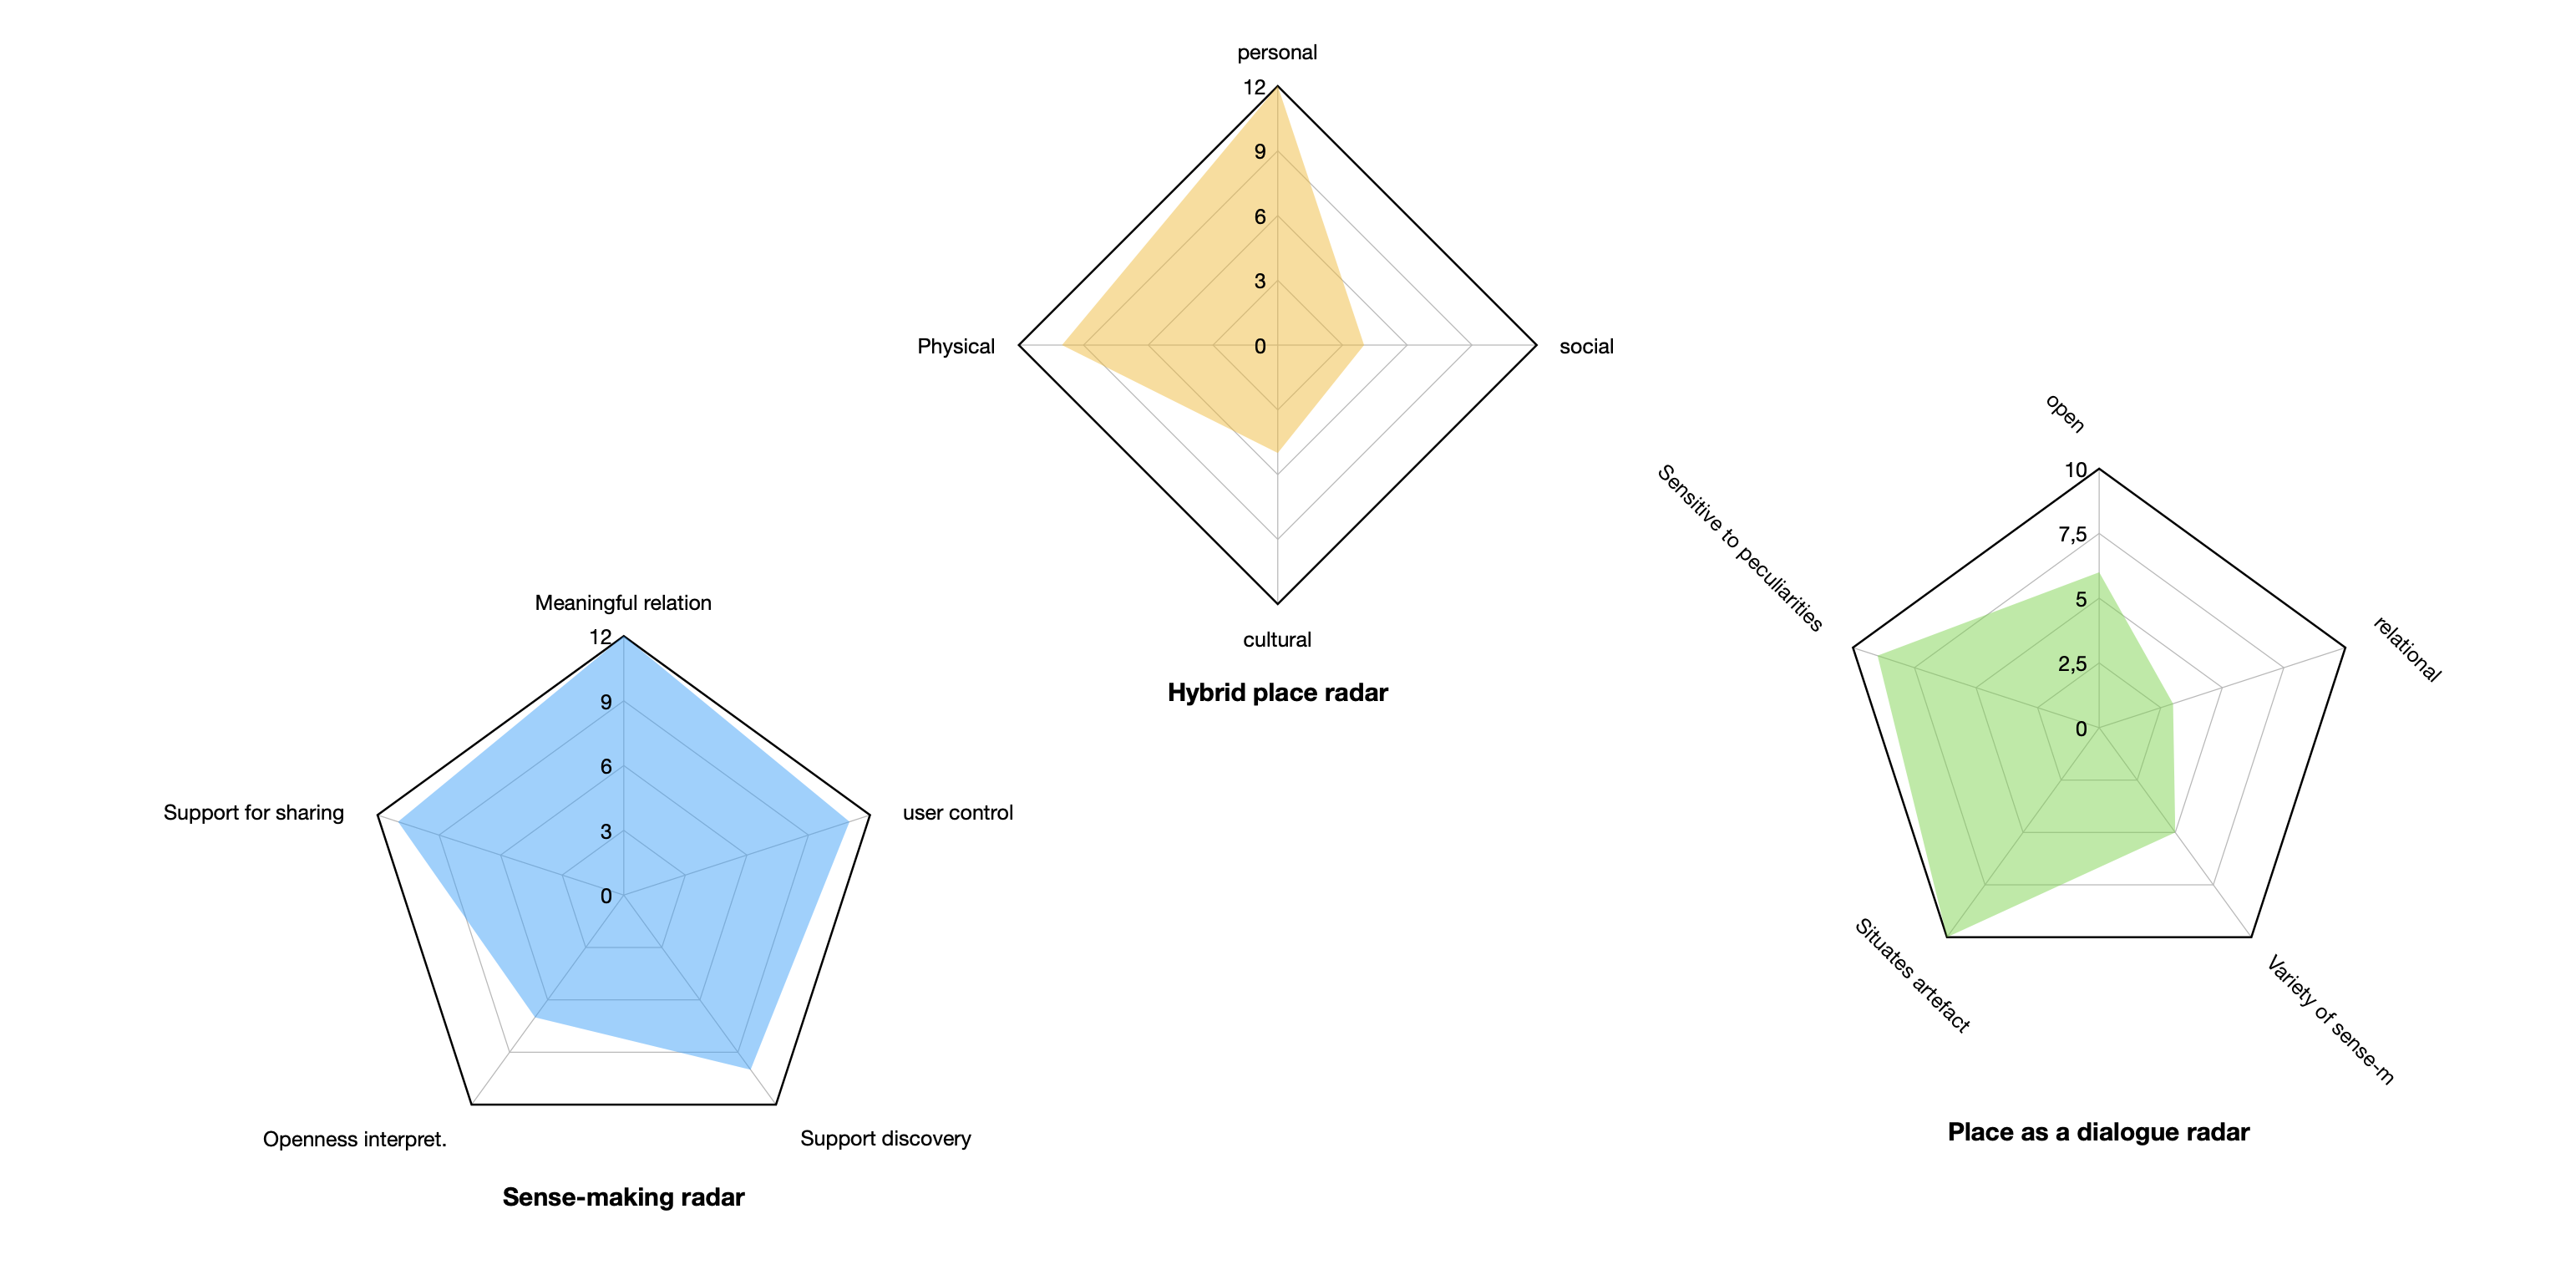
\includegraphics[width=13cm]{pictures/dataset/analysis_radars.png}
\centering 
\end{figure}

\emph{"Findings"}
\par

What I have learned by looking at the radar charts so far is how the different theories fulfill, or complement eachother. The way I have gone forward in looking at the radar charts is as following:
\par I'll start by looking at the hybrid place radar chart, noticing how the personal and physical dimension is fulfilled, while the social and cultural dimension is very little fulfilled. What does this mean? According to the Norwegian museum policy strategic thinking, it is wanted that museums transition from the personal dimension to the more social and cultural dimension. The fact that installations in my analysis shows presence in the physical dimension is positive, in terms of enabling the personal dimension, experience-wise, to involve more tangible or at least dynamic experiences in the museum space.
\par Then, if we shift focus for a second to look into the sense-making radar chart, we see that one of the corners that is fulfilled by almost all installations in this analysis - support for sharing is fulfilled. How come, that even though the social dimension is not fulfilled while almost all installations, in terms of sense-making have good support for sharing? 

\par Then again, we can look at what dialogic qualities the installations turns out to have little "relationalness", which is a dialogic principle/ quality that involves the Docents in the museum for example, or relational qualitites.






\section{Second iteration: looking for patterns}


\section{The role of prototyping in this thesis}
Research through design is a type of research practise where the researcher create artefact- or object prototypes to gain the necessary insight needed to drive and conduct the research project. Prototyping, or the use of prototypes can be used in a variety of ways, and in every stage throughout the project. In the field of human-computer interaction (HCI), software engineering and design, the term prototype is commonly used to signify a specific kind of object used in the design process (Lim et. al., 2008, p. 2). The prototypes are either physical or digital, and function as either a speculative solution, as a manifestation of a design idea, or to explore a design space - all in relation to the research scope and focus. Prototypes are the means by which designers organically and evolutionary learn, discover, generate and refine designs \cite{lim_anatomy_2008, p.2}. They are design-thinking enablers deeply embedded and immersed in design practise, not just as tools for evaluating or proving successes or failures of design outcomes (Lim et. al., 2008, p. 2).

In the search for a new way of thinking about prototypes and prototyping, based on the need for exploring and establishing a definition that differs from current approaches in software engineering contexts where engineers use prototypes to identify or satisfy requirements: Lim et. al., conceptualise prototypes as tools for traversing a design space where all possible design alternatives and their rationales can be explored (Lim et. al., 2008, p. 2). In that way, the prototype serves as a communicative manifestation, where the designer is enabled to communicate the rationales of their design decisions through the prototype (Lim et. al., 2008, p. 2). Prototypes stimulate reflections, and designers use them to frame, refine and discover possibilities in a design space (Lim et. al., 2008, p. 2). This new way of thinking about prototypes differs markedly from requirement-oriented approaches like software engineering, recognising design activities as flexible rather than rigid, reflective rather than prescriptive, and problem-setting rather than problem-solving (Schön, 1982). A design idea that satisfies all the identified requirements does not guarantee that it is the best design since a number of ways can meet each requirement (Lim et. al., 2008, p. 2). If the focus of prototyping is framing and exploring a design space, what matters is not identifying or satisfying requirements using prototypes but finding the manifestation that in its simplest form, filters the qualities in which designers are interested, without distorting the understanding of the whole (Lim et. al., 2008, p. 2). In order to support this perspective and to provide a stable foundation for the study of prototypes in HCI, Lim et. al. (2008) proposes a framework for conceptualising prototypes. The framework is an attempt to create an understanding of the nature of prototypes in general and to provide a language for articulating the characteristics of a particular prototype (Lim et. al., 2008, p. 3). Two fundamental aspects of prototyping form the basis of the framework:

1) prototypes are for traversing a design space, leading to the creation of meaningful knowledge about the final design as envisioned in the process of design, and
2) prototypes are purposefully formed manifestations of design ideas.
(Lim et. al., 2008, p. 3)

Will answer these:
What values are important in my context?
What is my design outcomes?
What is my design space?
Experience prototyping? Am I going to prototype an experience?
Why and how do I intend a particular prototype to support the design process?

In this thesis, the role of prototyping will be a proof of concept where the perspectives are manifested or represented. As a proof of concept of how I have used the framework/ thinking to design a meaningful interactive experience.
The prototypes main function is to work as a “mediator”, to facilitate for conversations with museumspeople or designer that will give insight to what the prototypes adresses.
